\documentclass[a4wide,10pt]{article}
\usepackage{a4wide}
\usepackage[applemac,utf8]{inputenc}
\usepackage[danish]{babel}
\usepackage[T1]{fontenc}
\usepackage{pdfsync}
\usepackage{amsmath,amssymb,amsfonts} 
\usepackage[pdftex]{graphicx}
\usepackage{wrapfig}
\usepackage{color}
\usepackage[small,bf]{caption}

\begin{document}
\title{DSP in hearing aids}
\author{Nis Sarup}
\date{\today}
\maketitle
\begin{center}
	SDU - Det Tekniske Fakultet\\
	Course: DSB\\
\end{center}
\newpage

\section{DSP in hearing aids} % (fold)
\label{sec:dsp_in_hearing_aids}

\subsection{Hearing impairment} % (fold)
\label{sub:hearing_impairment}
\begin{wrapfigure}{r}{0.5\textwidth}
	\vspace{-20pt}
	\begin{center}
		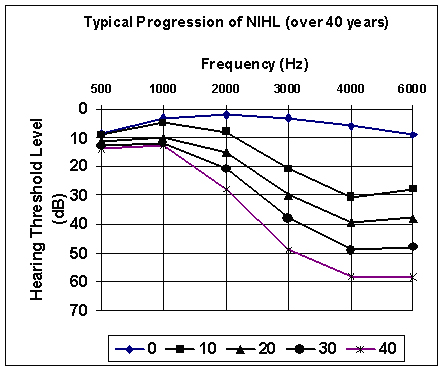
\includegraphics[width=0.48\textwidth]{images/nihl_graph.jpg}
	\end{center}
	\caption{NIHL: Noise Induce Hearing Loss}
	\vspace{-40pt}
\end{wrapfigure}
Our hearing can be impaired, either from natural causes or by accidents.


Causes can include:

\begin{itemize}
	\item Old age
	\item Heraditary causes
	\item Infections
	\item Acoustic trauma
\end{itemize}

Luckyly we are not reduced to use the old hearing horns or conversation tubes. We have DSP!
% subsection hearing_impairment (end)

\subsection{DSP to the rescue} % (fold)
\label{sub:dsp_to_the_rescue}
As can clearly be seen in the figure above, a straight amplification of all frequencies would be inappropriate as it would make frequencies in which the impaired had no loss of hearing sound too loud. Amplifying only the frequencies which the impaired have a hearing loss makes much more sense.

Singling out these frequencies and amplifying them can perhaps be done using analog devices, but it would mean a bulky hearing aid and one that could not easily be adopted to different types of hearing loss.

A digital hearing aid can be loaded with different profiles according to the specific need of its wearer.
% subsection dsp_to_the_rescue (end)
\end{document}